\documentclass{article}
\usepackage{lipsum}
\usepackage{geometry}
\usepackage{amsmath}
\usepackage{graphicx}
\linespread{1.5}
\author{Sergio Garcia-Rios 
	\thanks{Cornell University - Government}
	}
\title{Anxiously Preparing for a Final Paper: \\ 
A LaTeX Template for ARA Students}
\date{}



\maketitle

\begin{document}

\clearpage

\section{Introduction}
\lipsum[1-3]

\section{Theory and Hypotheses}
\lipsum[2]

% Comment here
\subsection{Hypotheses}
\lipsum[2] This here \footnote{This is the footnote stuff} is a footnote

\begin{itemize}
    \item Hypothesis 1: Lorem ipsum dolor sit amet, consectetuer adipiscing elit. Aenean commodo
    \item Hypothesis 2 Sed ut perspiciatis unde omnis iste natus error sit voluptatem accusantium doloremque
\end{itemize}


\lipsum[1]

\section{Data and Methods}

\lipsum[2]


% Table created by stargazer v.5.2.2 by Marek Hlavac, Harvard University. E-mail: hlavac at fas.harvard.edu
% Date and time: Mon, Apr 29, 2019 - 8:03:47 PM
\begin{table}[!htbp] \centering 
  \caption{Descriptive Statistics for Variables Used} 
  \label{tab: desc} 
\begin{tabular}{@{\extracolsep{5pt}}lccccccc} 
\\[-1.8ex]\hline 
\hline \\[-1.8ex] 
Statistic & \multicolumn{1}{c}{N} & \multicolumn{1}{c}{Mean} & \multicolumn{1}{c}{St. Dev.} & \multicolumn{1}{c}{Min} & \multicolumn{1}{c}{Pctl(25)} & \multicolumn{1}{c}{Pctl(75)} & \multicolumn{1}{c}{Max} \\ 
\hline \\[-1.8ex] 
Vote for Trump & 3,484 & 0.389 & 0.488 & 0.000 & 0.000 & 1.000 & 1.000 \\ 
Male & 4,219 & 0.471 & 0.499 & 0.000 & 0.000 & 1.000 & 1.000 \\ 
Income & 4,069 & 15.387 & 8.080 & 1.000 & 9.000 & 22.000 & 28.000 \\ 
Age & 4,150 & 49.576 & 17.581 & 18.000 & 34.000 & 63.000 & 90.000 \\ 
Conservative & 4,248 & 4.137 & 1.411 & 1.000 & 4.000 & 5.000 & 7.000 \\ 
Education & 4,232 & 11.264 & 3.568 & 1.000 & 9.000 & 13.000 & 90.000 \\ 
Sexism & 4,154 & 2.675 & 1.165 & 1.000 & 2.000 & 3.000 & 5.000 \\ 
Oppose Aff Action & 4,224 & 2.261 & 0.750 & 1.000 & 2.000 & 3.000 & 3.000 \\ 
Immigration Axiety & 3,622 & 3.473 & 1.139 & 1.000 & 3.000 & 4.750 & 5.000 \\ 
Economic Anxiety & 3,639 & 3.031 & 1.017 & 1.000 & 2.000 & 4.000 & 5.000 \\ 
White & 4,211 & 0.810 & 0.392 & 0.000 & 1.000 & 1.000 & 1.000 \\ 
\hline \\[-1.8ex] 
\end{tabular} 
\end{table} 

\lipsum[3]

\subsection{Models and specification}

\lipsum[4]


\begin{multline}
  \operatorname{Pr}(\text{Vote} = 1 \mid \text{H, T})\\
 = \frac{\exp(\beta_{0} + \beta_{1} \text{Gender} + \beta_{2} \text{Age} + \dots +
    \beta_{12} \text{immigration)} }{1 + \exp(\beta_{0} + \beta_{1} \text{Gender} + \beta_{2} \text{Age} +
\dots + \beta_{12 }\text{immigration})} \label{eq:glm1} 
\end{multline}



\lipsum[5]



\section{Results}

\lipsum[2]

I can reference Table \ref{tab: regs} here and can reference Figure \ref{fig: ame} and Equation \ref{eq:glm1}



% Table created by stargazer v.5.2.2 by Marek Hlavac, Harvard University. E-mail: hlavac at fas.harvard.edu
% Date and time: Mon, Apr 29, 2019 - 12:50:03 PM
\begin{table}[!htbp] \centering 
  \caption{Logistic Regression: Trump something something} 
  \label{tab: regs} 
\begin{tabular}{@{\extracolsep{5pt}}lccc} 
\\[-1.8ex]\hline 
\hline \\[-1.8ex] 
 & \multicolumn{3}{c}{\textit{Dependent variable:}} \\ 
\cline{2-4} 
\\[-1.8ex] & \multicolumn{3}{c}{Vote for Trump} \\ 
\\[-1.8ex] & (1) & (2) & (3)\\ 
\hline \\[-1.8ex] 
 Male & 0.120 (0.096) & 0.123 (0.104) & 0.187 (0.115) \\ 
  Income & $-$0.008 (0.007) & $-$0.009 (0.007) & $-$0.004 (0.008) \\ 
  Age & 0.006$^{**}$ (0.003) & 0.009$^{***}$ (0.003) & 0.003 (0.003) \\ 
  Conservative & 1.188$^{***}$ (0.046) & 1.205$^{***}$ (0.050) & 1.061$^{***}$ (0.056) \\ 
  Education & $-$0.035$^{*}$ (0.020) & $-$0.023 (0.018) & 0.006 (0.017) \\ 
  Sexism &  &  & 0.306$^{***}$ (0.052) \\ 
  Oppose Aff Action &  &  & 0.529$^{***}$ (0.086) \\ 
  Immigration Axiety &  &  & 0.798$^{***}$ (0.059) \\ 
  Economic Anxiety &  & 0.123$^{**}$ (0.052) & $-$0.029 (0.058) \\ 
  White & 2.150$^{***}$ (0.167) & 2.042$^{***}$ (0.181) & 1.837$^{***}$ (0.196) \\ 
  Constant & $-$7.253$^{***}$ (0.356) & $-$7.891$^{***}$ (0.439) & $-$11.788$^{***}$ (0.566) \\ 
 \hline \\[-1.8ex] 
Observations & 3,207 & 2,772 & 2,721 \\ 
Log Likelihood & $-$1,383.997 & $-$1,188.652 & $-$1,004.843 \\ 
Akaike Inf. Crit. & 2,781.994 & 2,393.304 & 2,031.685 \\ 
\hline 
\hline \\[-1.8ex] 
\textit{Note:}  & \multicolumn{3}{r}{$^{*}$p$<$0.1; $^{**}$p$<$0.05; $^{***}$p$<$0.01} \\ 
\end{tabular} 
\end{table} 


\lipsum[5-6]


\begin{figure}
\centering
\caption{This is the title for this figure}
\label{fig: ame}
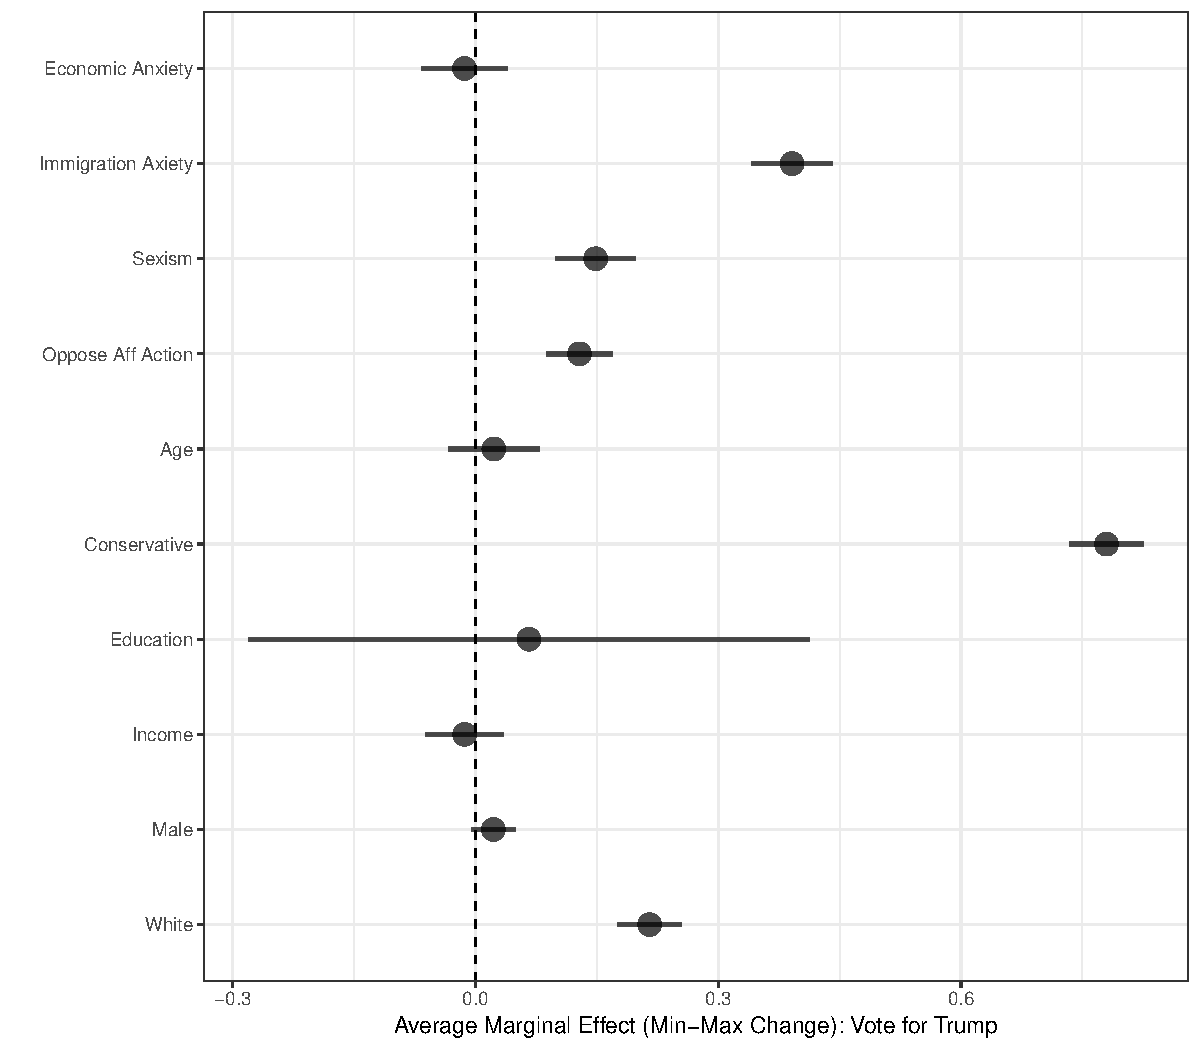
\includegraphics[scale=.6]{ame_plot}
\end{figure}

\lipsum[5]


\begin{figure}
\centering
\caption{This is the title for this figure}
\label{fig: preds}
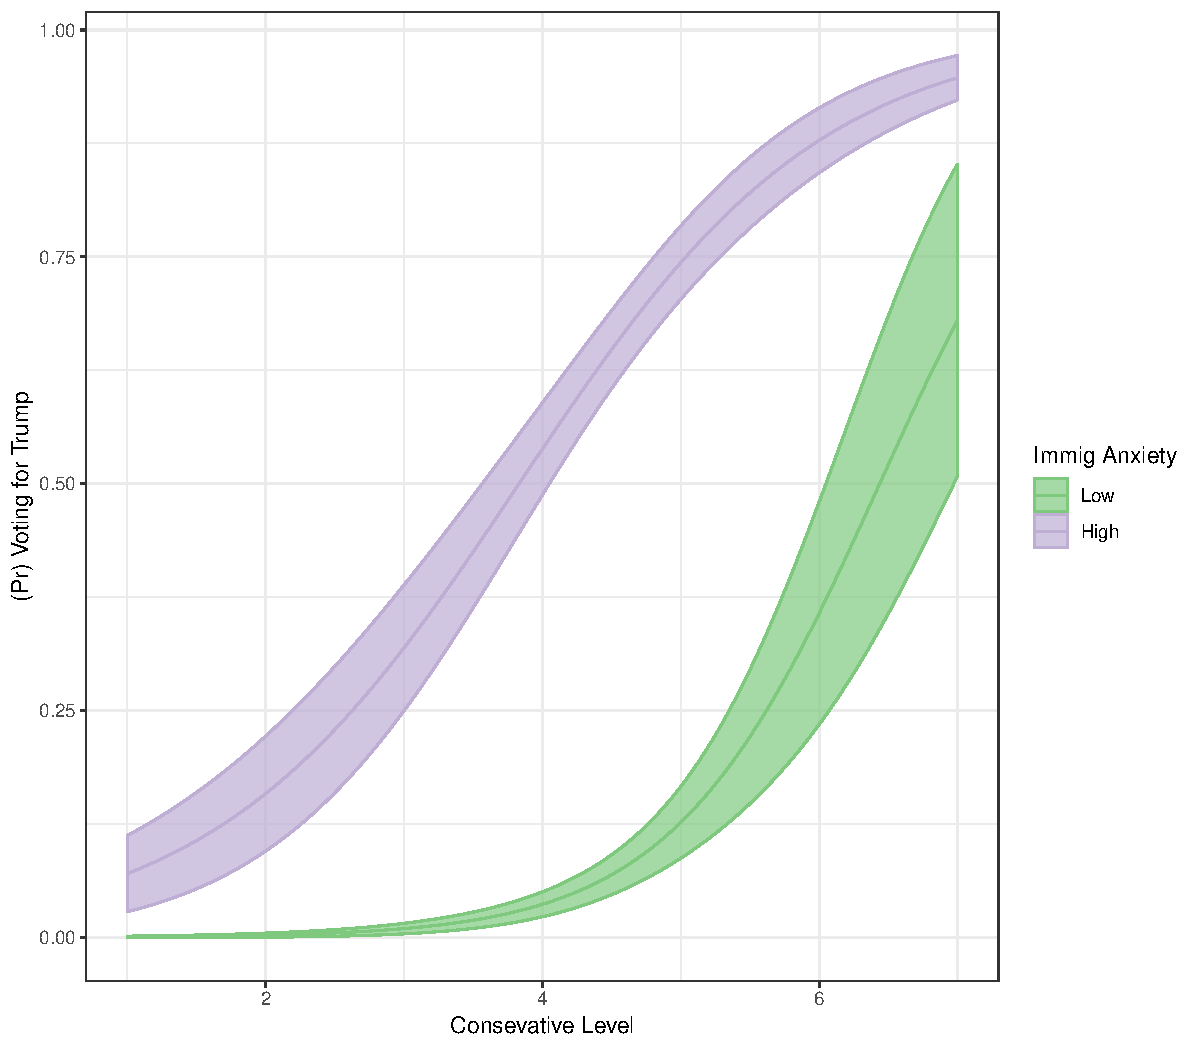
\includegraphics[scale=.6]{preds}
\end{figure}

\lipsum[8]

\section{Conclusion}

\lipsum[20-22]




\end{document}


































































